Use RF fields in a linear quadrupole ion trap (LQT) to trap charged particles spatially.\cite{Wolfgang1990} Consider a 3 dimensional potential that could trap a particle, we may assume the form:
\begin{align*}
	\Phi = \frac{\Phi}{r_0^2} \sum_{i=1}^3 \alpha_i r_i^2
\end{align*}
Where $r_0$ is the distance to the potential surfaces and $r_{1,2,3}$ correspond to $x$, $y$, and $z$ respectively. But by Laplace's equation, $\Delta \Phi = 0$, we don't get a confining potential as one of the terms $\alpha_i$ must be negative, leading to a saddle-like potential. To get around this, we may vary the potential in time to create a pseudo-potential that can confine a subset of ions:
\begin{equation*}
	\Phi_0(t) = V_{DC} + V_{rf} \cos(\Omega_{rf} t)
\end{equation*}
Solving for the equations of motion, we find:
\begin{equation}
	\ddot{r}_i + \frac{2 \alpha_i e}{m r_0^2}(V_{DC} + V_{AC} \cos(\Omega_{rf} t))r_0 = 0
\end{equation}
To solve this, we make changes of variable:
\begin{align}
	a & = \frac{8eV_{DC}}{mr_0^2\Omega_{rf}^2} \label{eq: a param} \\
	q & = \frac{4eV_{DC}}{mr_0^2\Omega_{rf}^2} \label{eq: q param} \\
	\tau & = \frac{1}{2}\Omega_{rf} t \nonumber
\end{align}
To then find the characteristic Mathieu equation:
\begin{equation}
	\frac{\partial^2 u}{\partial \tau^2} + (a - 2q \cos(2 \tau))u = 0
	\label{eq: Mathieu diffeq}
\end{equation}
A diagram showing stable solutions to equation \ref{eq: Mathieu diffeq} with the experimental trap values is shown in figure \ref{fig: stability}. To provide full 3 dimensional trapping, DC end cap voltages of around 200 V are applied to contain the ions axially.

Considering our linear quadrupole trap, where we have radial symmetry, the conditions for the $x$ and $y$ orientations are the same, where $a_x = a_y = -\frac{1}{2}a_z$ as well as $q_x = q_y = -\frac{1}{2}q_z$. As long as we are in a regime where $a \ll q^2 \ll 1$, we can approximate the pseudo-potential as a harmonic oscillator where multiples of the secular frequency are the allowed modes.
\begin{equation}
	\omega_i = \gamma_i \frac{\Omega_{rf}}{2}
	\label{eq: secular freq}
\end{equation}
Where $\gamma_i = \sqrt{a_i + \frac{q_i^2}{2}}$. Inside this harmonic potential, the ions may move around up until the point at which they would hit the trap rods. Keeping with the harmonic potential approximation, we can characterize the maximum energy an ion may have in the trap to be when the energy of the ion at the condition where it would be displaced far enough to hit a rod.
\begin{equation}
	E_0 = \frac{m}{2e} \omega_{sec}^2r_0^2
	\label{eq: trap depth}
\end{equation}
Compiling the relevant trap parameters and using equations \cref{eq: secular freq,eq: trap depth}:

\begin{table}[H]
	\centering
	\begin{tabular}{|c|c|}
		\hline
		Parameter & Value \\
		\hline
		$r_0$ & 6.85 mm \\
		$\Omega_{rf}$ & $(2 \pi) 3$ MHz \\
		$V_{DC}$ & 2 V \\
		$V_{rf}$ & 250 V \\
		$\omega_{sec}$ & 83 kHz \\
		$E_0(m/z=9)$ & 3 eV \\
		\hline
	\end{tabular}
	\caption{Experimental trap parameters predominantly used in this thesis.}
	\label{tab: trap params}
\end{table}

\begin{figure}[H]
	\centering
	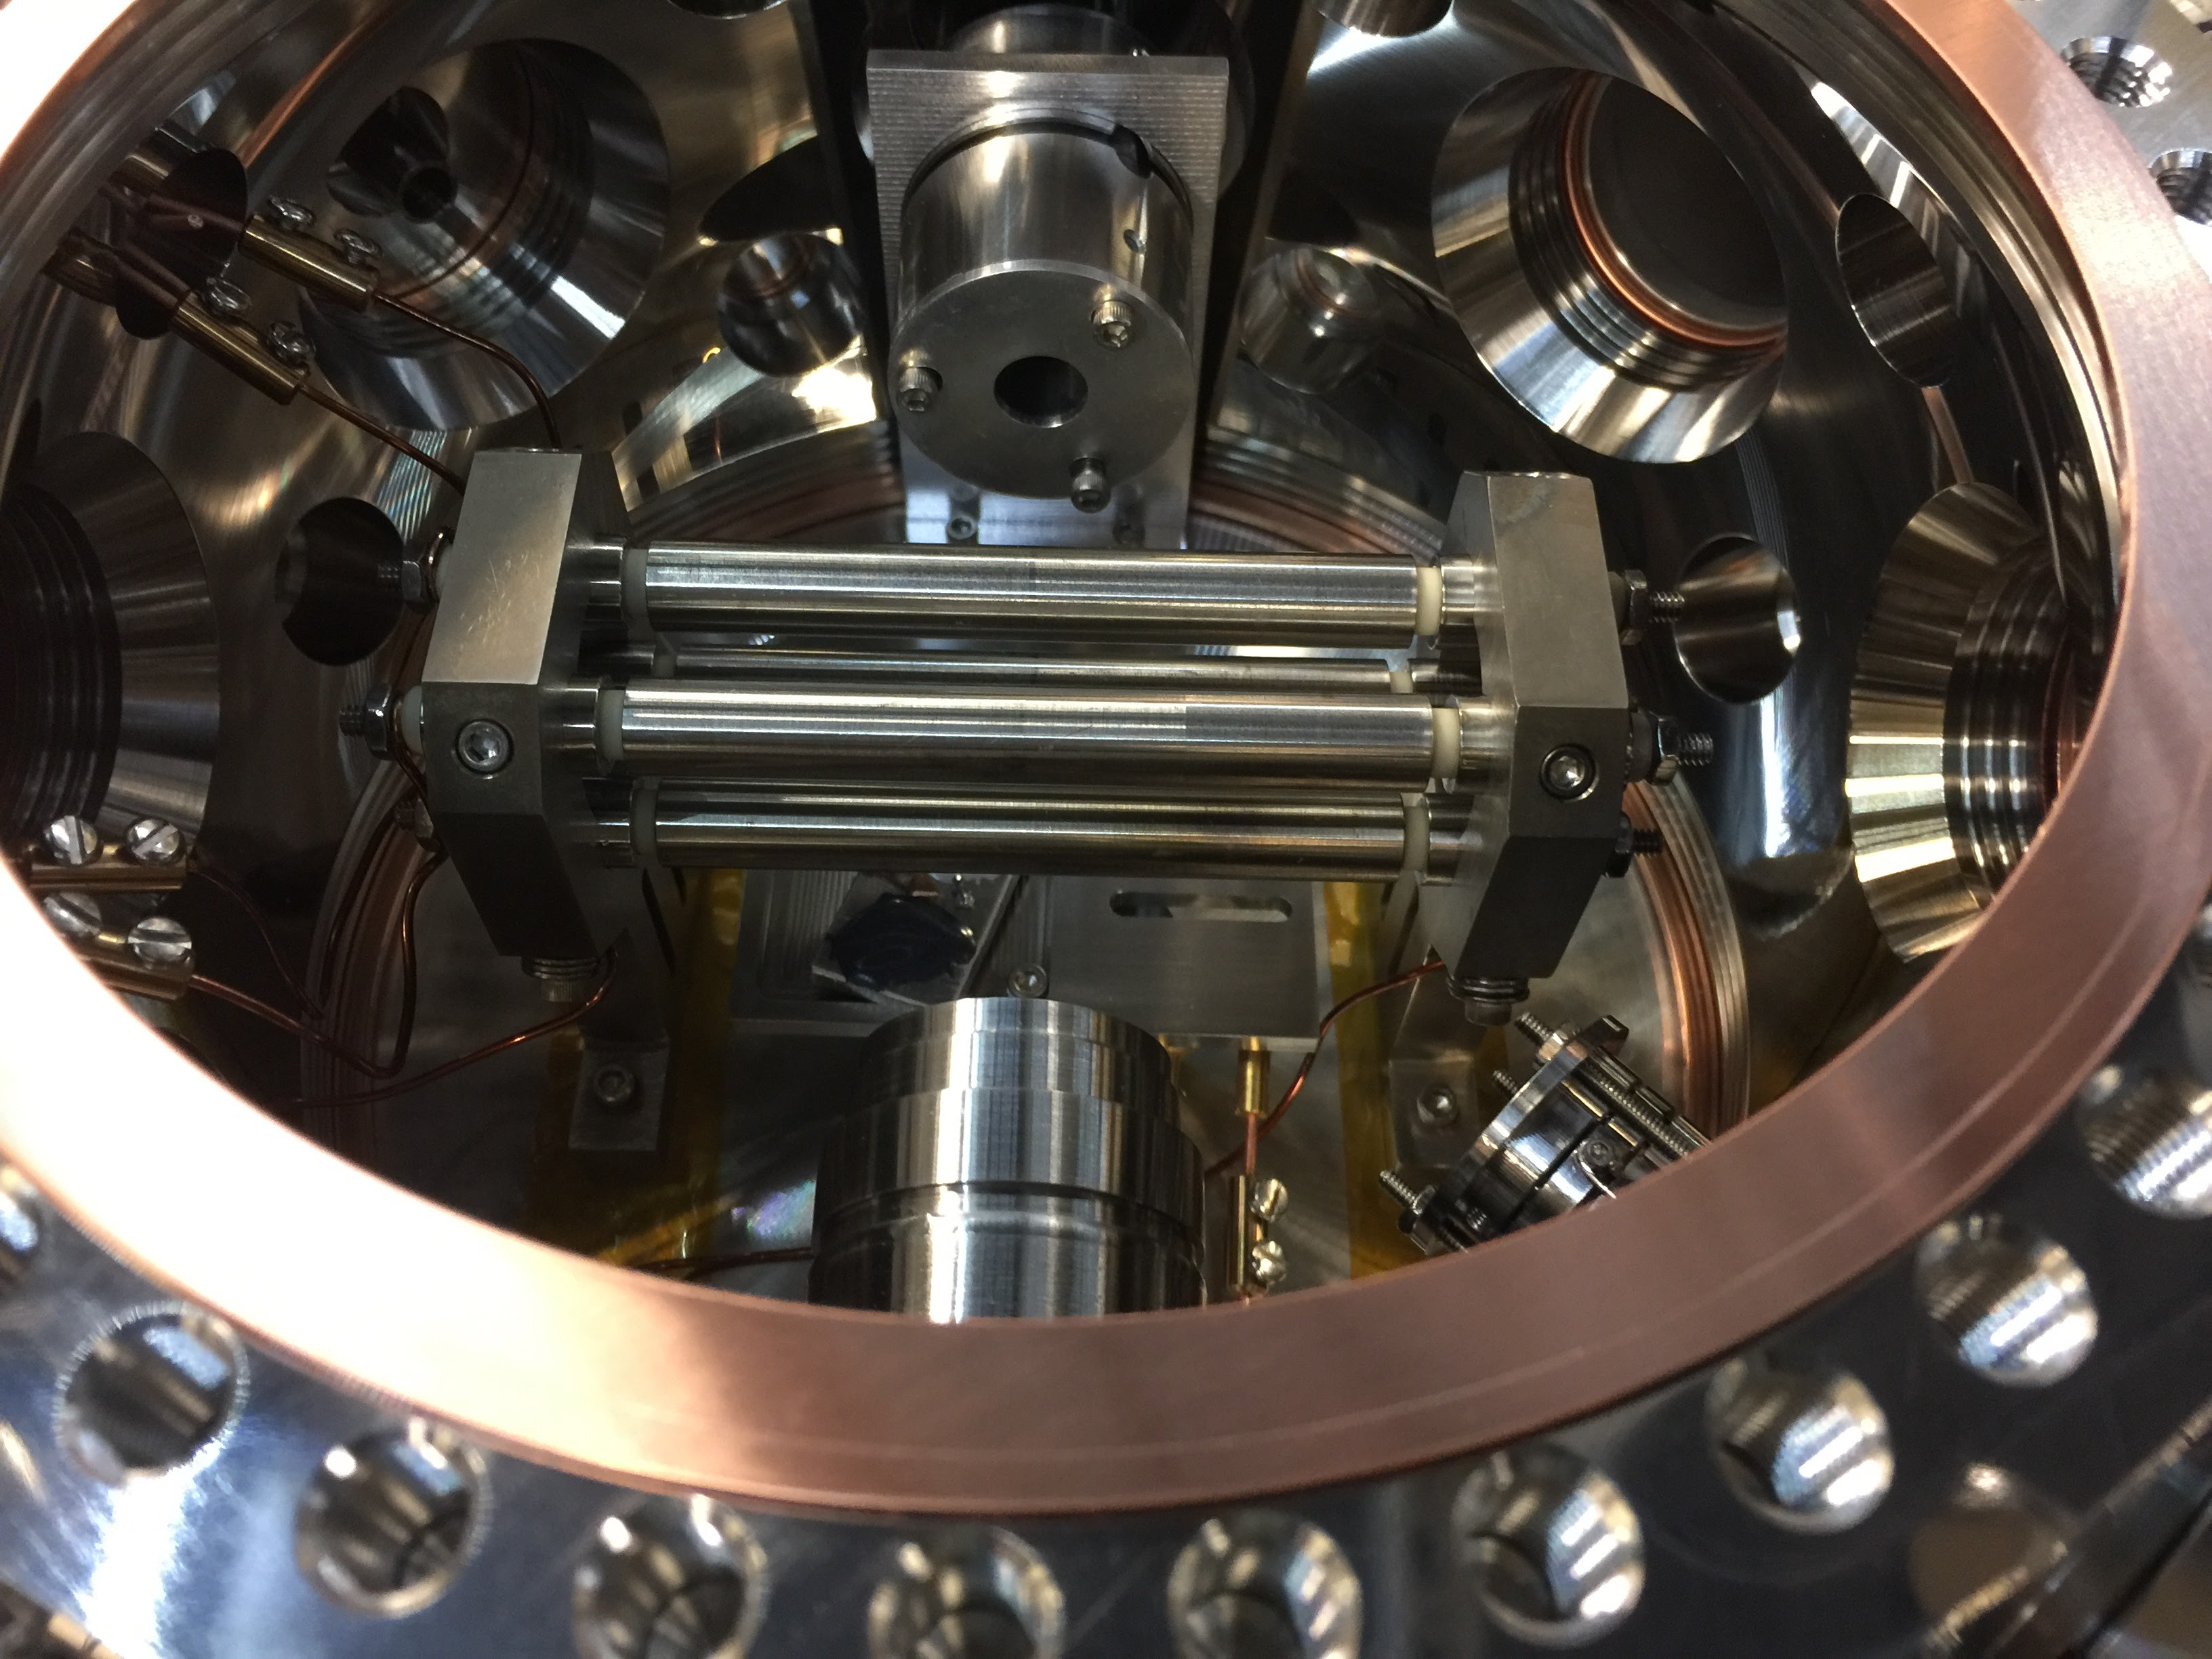
\includegraphics[width=0.8\textwidth]{images/ion_trap.jpg}
	\caption{The ion trap inside of the experimental vacuum chamber. An Einzel lens and imaging objective are seen on the vertical axis.}
\end{figure}

\begin{figure}[H]
	\centering
	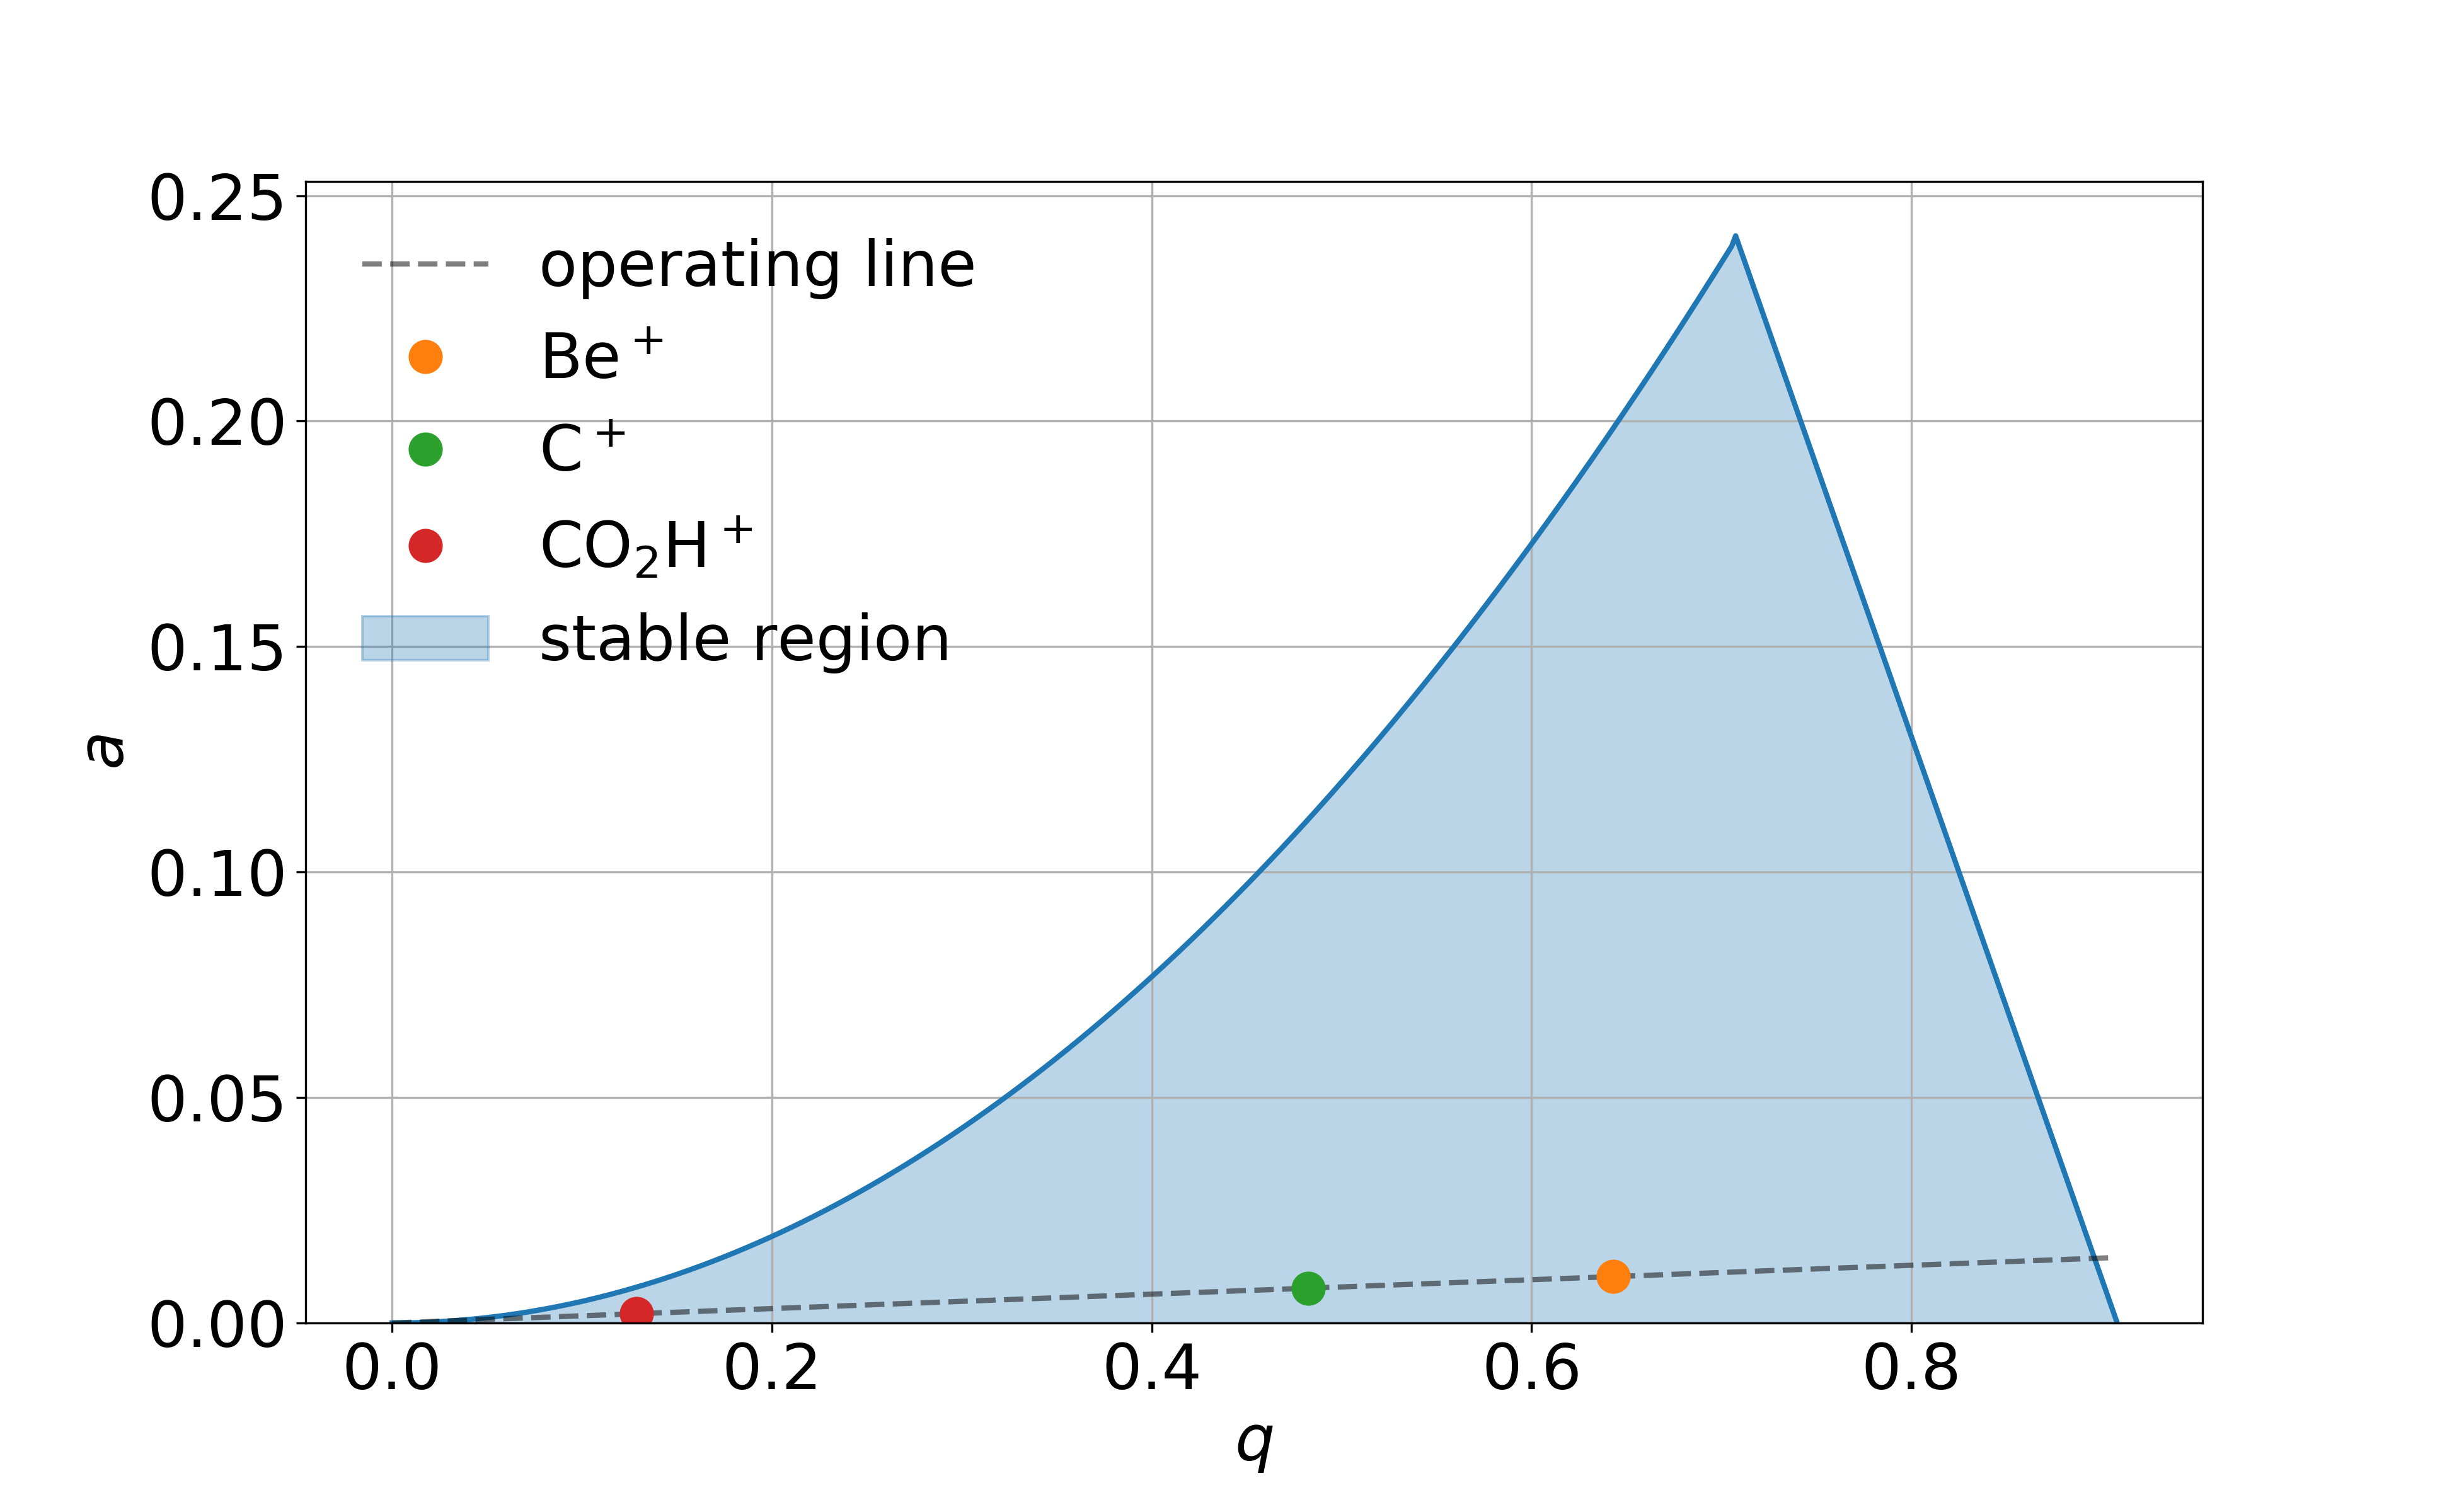
\includegraphics[width=0.8\textwidth]{images/stability.png}
	\caption{Stability diagram of the experimental ion trap with parameters defined in table \ref{tab: trap params}. The trap is set up to be stable for ions of interest, including high mass reaction products, from \ce{Be+}, and \ce{C+} at $m/z=$9, 12 to \ce{CO2H+} at $m/z=45$.}
	\label{fig: stability}
\end{figure}

%The differential equation has stable solutions, which can be shown to be.\cite{Ghosh1995}
%
%\begin{equation}
%	u(\tau) = A \sum C_{2n} \cos((2n+\beta) u) + B\sum C_{2n} \sin((2n + \beta) u)
%\end{equation}
%
%$A$ and $B$ are integration constants that are determined by the initial conditions of the ion, and constants and $C_{2n}$ \todo{talk about this more}.